\section{CƠ SỞ LÝ THUYẾT}\label{sec:co_so_ly_thuyet}

\subsection{Tổng quan về mạng Campus}

Mạng Campus là hệ thống mạng nội bộ được triển khai trong phạm vi một khuôn viên tổ chức như trường đại học, viện nghiên cứu, doanh nghiệp hoặc cơ quan hành chính. Trong môi trường trường đại học, mạng Campus đóng vai trò kết nối các khoa, phòng ban, phòng học, phòng máy, thư viện, khu vực hành chính, hệ thống máy chủ nội bộ và hệ thống truy cập không dây. Khác với một mạng LAN nhỏ, mạng Campus thường có số lượng người dùng lớn, nhiều nhóm thiết bị khác nhau và yêu cầu cao về hiệu năng, tính ổn định, khả năng mở rộng cũng như bảo mật.

Đối với đề tài này, mạng Campus được xem là hạ tầng nền tảng phục vụ hoạt động học tập, nghiên cứu và quản trị nhà trường. Hệ thống cần bảo đảm người dùng có thể truy cập các dịch vụ dùng chung như Internet, máy chủ học tập, hệ thống quản lý đào tạo, máy in, kho dữ liệu và các dịch vụ nội bộ khác. Đồng thời, mạng phải phân tách rõ ràng giữa các nhóm người dùng như sinh viên, giảng viên, khách, phòng máy và bộ phận quản trị để hạn chế truy cập trái phép và giảm ảnh hưởng khi xảy ra sự cố.

Một mạng Campus hiện đại thường phải đáp ứng các yêu cầu chính sau: băng thông đủ lớn cho lưu lượng học tập và nghiên cứu; độ trễ thấp đối với các dịch vụ thời gian thực; khả năng dự phòng khi một đường truyền hoặc thiết bị gặp lỗi; chính sách bảo mật nhất quán giữa các khu vực; khả năng giám sát tập trung; và khả năng mở rộng khi số lượng người dùng, VLAN hoặc cơ sở đào tạo tăng lên. Đây cũng là lý do đề tài định hướng kết hợp mô hình mạng phân cấp truyền thống với các công nghệ quản lý hiện đại như SDN và SD-WAN.

\subsection{Mô hình mạng phân cấp Core--Distribution--Access}

Mô hình Core--Distribution--Access là kiến trúc phổ biến trong thiết kế mạng Campus vì chia hệ thống thành các tầng chức năng rõ ràng. Cách phân tầng này giúp quá trình thiết kế, vận hành và mở rộng mạng trở nên có tổ chức hơn, đồng thời giảm độ phức tạp khi cần xử lý sự cố hoặc bổ sung khu vực mới.

\begin{figure}[H]
    \centering
    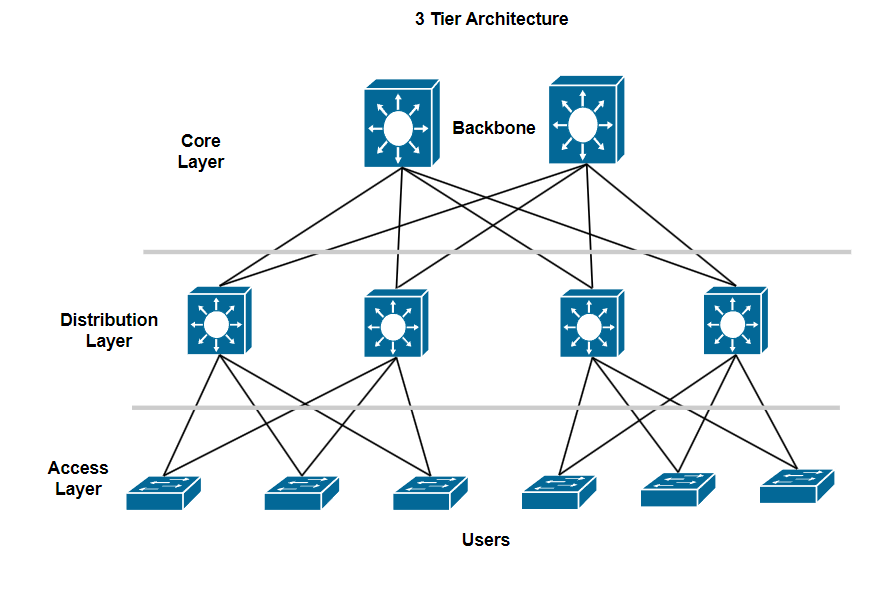
\includegraphics[width=0.80\textwidth]{image/mohinh.png}
    \caption{Mô hình mạng phân cấp Core--Distribution--Access}
    \label{fig:core_distribution_access}
\end{figure}

Tầng Access là tầng gần người dùng cuối nhất, nơi kết nối trực tiếp máy tính, điện thoại IP, camera, máy in, thiết bị Wi-Fi và các thiết bị đầu cuối khác. Tại tầng này, quản trị viên thường cấu hình cổng access, gán VLAN, áp dụng các chính sách bảo mật cơ bản, giới hạn truy cập và thu thập thông tin trạng thái kết nối. Vì tầng Access có số lượng cổng lớn nên tính dễ quản lý và khả năng chuẩn hóa cấu hình là yêu cầu quan trọng.

Tầng Distribution đóng vai trò tập trung lưu lượng từ nhiều switch Access, thực hiện định tuyến liên VLAN, áp dụng ACL, tổng hợp kết nối và triển khai các cơ chế dự phòng. Đây là tầng trung gian giúp kiểm soát chính sách giữa các vùng mạng khác nhau, ví dụ giữa VLAN sinh viên và VLAN máy chủ hoặc giữa VLAN khách và hệ thống nội bộ. Trong nhiều thiết kế Campus, tầng Distribution cũng là nơi đặt gateway mặc định cho các VLAN người dùng.

Tầng Core là xương sống của mạng Campus, chịu trách nhiệm chuyển tiếp lưu lượng tốc độ cao giữa các khu vực lớn trong hệ thống. Tầng Core cần được thiết kế đơn giản, ổn định và có khả năng dự phòng cao. Các thiết bị tại tầng này thường hạn chế xử lý chính sách phức tạp để ưu tiên tốc độ chuyển tiếp và độ tin cậy. Khi mạng có nhiều tòa nhà hoặc nhiều khu vực chức năng, tầng Core giúp kết nối các khối Distribution lại với nhau theo mô hình tập trung.

Việc áp dụng mô hình phân cấp giúp đề tài xây dựng được một topology rõ ràng: người dùng kết nối ở tầng Access, chính sách và định tuyến liên VLAN được xử lý ở tầng Distribution, còn tầng Core bảo đảm kết nối tốc độ cao giữa các vùng. Đây là nền tảng để triển khai thêm SDN Controller nhằm quản lý tập trung và SD-WAN nhằm kết nối nhiều cơ sở.

\subsection{VLAN và phân đoạn mạng}

\begin{figure}[H]
    \centering
    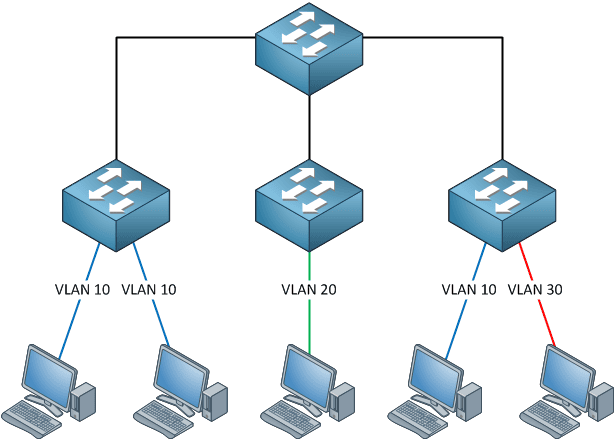
\includegraphics[width=0.80\textwidth]{image/vlan.png}
    \caption{Minh họa VLAN và phân đoạn mạng}
    \label{fig:vlan_phan_doan_mang}
\end{figure}

VLAN là kỹ thuật chia một hạ tầng switch vật lý thành nhiều mạng logic độc lập. Mỗi VLAN tương ứng với một miền quảng bá riêng, nhờ đó lưu lượng broadcast được giới hạn trong phạm vi cần thiết và các nhóm người dùng được tách biệt về mặt logic. Trong mạng Campus, VLAN thường được dùng để phân chia theo chức năng như VLAN sinh viên, VLAN giảng viên, VLAN hành chính, VLAN phòng máy, VLAN máy chủ, VLAN Wi-Fi khách và VLAN quản trị thiết bị.

Cổng access là cổng kết nối thiết bị đầu cuối và thường thuộc về một VLAN duy nhất. Ngược lại, cổng trunk được dùng để truyền lưu lượng của nhiều VLAN giữa các switch hoặc giữa switch và thiết bị định tuyến. Khi lưu lượng đi qua đường trunk, mỗi frame được gắn thẻ VLAN để thiết bị nhận biết frame đó thuộc mạng logic nào. Thiết kế trunk hợp lý giúp nhiều VLAN có thể cùng sử dụng một liên kết vật lý nhưng vẫn được phân tách về mặt logic.

Do các VLAN là các mạng khác nhau, thiết bị trong VLAN này muốn giao tiếp với VLAN khác cần có cơ chế định tuyến liên VLAN. Cơ chế này có thể được thực hiện bằng router, switch lớp 3 hoặc thiết bị gateway tại tầng Distribution. Trong đề tài, định tuyến liên VLAN là thành phần quan trọng để kiểm soát đường đi của lưu lượng giữa các khu vực chức năng. Ví dụ, VLAN sinh viên có thể được phép truy cập Internet và hệ thống học tập, nhưng không được truy cập trực tiếp VLAN quản trị thiết bị.

Phân đoạn mạng bằng VLAN không chỉ cải thiện hiệu năng mà còn tăng tính bảo mật. Khi kết hợp VLAN với ACL, NAC hoặc chính sách trên SDN Controller, hệ thống có thể kiểm soát quyền truy cập theo vai trò người dùng, vị trí kết nối hoặc loại dịch vụ. Đây là cơ sở để xây dựng chính sách mạng phù hợp với môi trường trường đại học có nhiều nhóm người dùng và mức độ tin cậy khác nhau.

\subsection{Định tuyến và dịch vụ mạng nền tảng}

\begin{figure}[H]
    \centering
    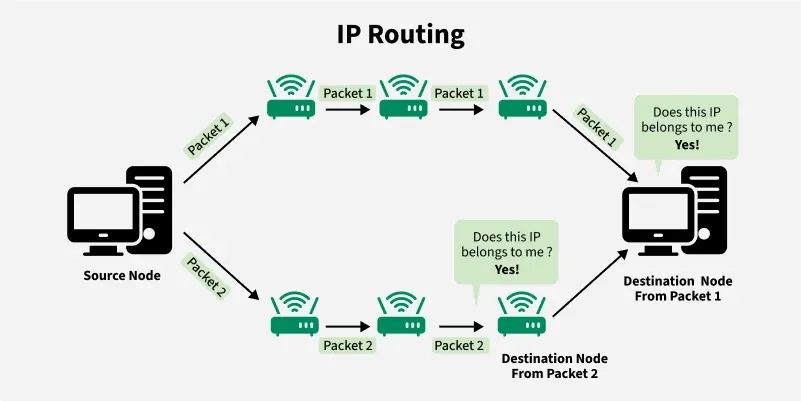
\includegraphics[width=0.80\textwidth]{image/iprouting.png}
    \caption{Minh họa định tuyến IP trong mạng}
    \label{fig:ip_routing}
\end{figure}

Định tuyến là quá trình xác định đường đi cho gói tin từ mạng nguồn đến mạng đích. Trong mạng Campus, định tuyến thường xuất hiện ở tầng Distribution hoặc Core để kết nối các VLAN, vùng máy chủ, vùng quản trị và đường ra Internet. Một thiết kế định tuyến tốt cần bảo đảm đường đi ổn định, dễ mở rộng và có khả năng hội tụ nhanh khi liên kết gặp sự cố.

OSPF là giao thức định tuyến nội bộ thường được dùng trong các hệ thống mạng có quy mô vừa và lớn. OSPF hoạt động theo cơ chế trạng thái liên kết, cho phép các router hoặc switch lớp 3 trao đổi thông tin topology và tự tính toán đường đi tối ưu. Ưu điểm của OSPF là hỗ trợ phân vùng, hội tụ tương đối nhanh và phù hợp với mô hình mạng phân cấp. Trong đề tài, OSPF có thể được sử dụng giữa các thiết bị Distribution và Core để tự động cập nhật đường đi thay vì cấu hình định tuyến tĩnh cho toàn bộ hệ thống.

DHCP là dịch vụ cấp phát địa chỉ IP tự động cho thiết bị đầu cuối. Trong môi trường Campus, DHCP giúp giảm khối lượng cấu hình thủ công, hạn chế trùng địa chỉ IP và hỗ trợ quản trị tập trung theo từng VLAN. Mỗi VLAN có thể được cấu hình một dải địa chỉ riêng, gateway mặc định, DNS và thời gian thuê địa chỉ phù hợp. Đối với các thiết bị hạ tầng như switch, router, server hoặc Controller, địa chỉ IP tĩnh vẫn nên được sử dụng để dễ quản lý và giám sát.

DNS là dịch vụ phân giải tên miền hoặc tên máy chủ thành địa chỉ IP. Trong mạng nội bộ, DNS giúp người dùng truy cập dịch vụ bằng tên dễ nhớ thay vì địa chỉ IP. Ngoài DNS, hệ thống Campus còn cần các dịch vụ nền tảng khác như NTP để đồng bộ thời gian, Syslog để ghi nhận sự kiện, SNMP hoặc giao thức giám sát tương đương để theo dõi trạng thái thiết bị. Các dịch vụ này hỗ trợ đáng kể cho vận hành, kiểm thử và đánh giá hệ thống.

\subsection{Cơ chế bảo mật và dự phòng trong mạng Campus}

Bảo mật mạng Campus cần được triển khai theo nhiều lớp, từ phân đoạn mạng, kiểm soát truy cập, bảo vệ cổng kết nối đến giám sát lưu lượng. ACL là một cơ chế phổ biến dùng để cho phép hoặc từ chối lưu lượng dựa trên địa chỉ nguồn, địa chỉ đích, giao thức và cổng dịch vụ. Khi đặt ACL tại tầng Distribution hoặc gateway liên VLAN, quản trị viên có thể kiểm soát chặt chẽ luồng dữ liệu giữa các nhóm người dùng.

Một nguyên tắc quan trọng là chỉ cho phép những truy cập cần thiết cho mục tiêu nghiệp vụ. Ví dụ, VLAN sinh viên có thể truy cập máy chủ học tập và Internet nhưng không được truy cập vùng quản trị; VLAN khách chỉ được truy cập Internet; VLAN quản trị được phép truy cập giao diện quản lý thiết bị; còn VLAN máy chủ chỉ mở các dịch vụ cần thiết. Cách tiếp cận này giúp giảm bề mặt tấn công và hạn chế lan truyền sự cố trong mạng nội bộ.

Ở tầng Access, các kỹ thuật như giới hạn địa chỉ MAC, tắt cổng không sử dụng, cấu hình VLAN riêng cho khách và kiểm soát truy cập theo người dùng giúp tăng mức an toàn cho điểm kết nối đầu cuối. Với hệ thống Wi-Fi, việc tách SSID theo nhóm người dùng và ánh xạ từng SSID vào VLAN phù hợp giúp chính sách truy cập nhất quán giữa mạng có dây và không dây.

Dự phòng là yêu cầu không thể thiếu trong mạng Campus vì sự cố tại một liên kết hoặc thiết bị có thể ảnh hưởng đến nhiều người dùng. STP hoặc RSTP được sử dụng để ngăn vòng lặp lớp 2 khi tồn tại nhiều đường kết nối dự phòng giữa các switch. Ở lớp 3, OSPF có thể tự động chọn đường thay thế khi một liên kết bị lỗi. Ngoài ra, thiết kế có thể sử dụng liên kết kép, thiết bị Core/Distribution dự phòng và nguồn điện dự phòng để tăng tính sẵn sàng của hệ thống.

\subsection{Công nghệ SDN}

SDN (Software-Defined Networking) là mô hình mạng dựa trên phần mềm, trong đó mặt phẳng điều khiển (control plane) được tách khỏi mặt phẳng chuyển tiếp dữ liệu (data plane). Trong mạng truyền thống, mỗi router hoặc switch thường tự đảm nhiệm cả việc tính toán đường đi, lưu giữ bảng định tuyến và chuyển tiếp gói tin. Với SDN, các quyết định điều khiển được tập trung tại bộ điều khiển SDN Controller, còn thiết bị mạng ở phía dưới chủ yếu thực hiện chuyển tiếp theo các quy tắc hoặc luồng dữ liệu do Controller cung cấp.

Cách tiếp cận này giúp trừu tượng hóa hạ tầng mạng và làm cho quá trình quản trị trở nên linh hoạt hơn. Quản trị viên có thể giám sát topology, điều chỉnh chính sách lưu lượng, thay đổi đường đi hoặc triển khai dịch vụ mạng từ một điểm quản lý tập trung thay vì cấu hình thủ công trên từng thiết bị riêng lẻ. Nhờ đó, SDN phù hợp với các hệ thống cần mở rộng nhanh, thay đổi chính sách thường xuyên và yêu cầu khả năng tự động hóa cao như trung tâm dữ liệu, điện toán đám mây, mạng doanh nghiệp và mạng Campus.

\subsubsection{Kiến trúc SDN ba lớp}

Kiến trúc SDN thường được mô tả theo ba lớp chính: lớp ứng dụng, lớp điều khiển và lớp hạ tầng. Ba lớp này phối hợp với nhau thông qua các giao diện lập trình để triển khai chính sách mạng một cách tập trung và nhất quán.

\begin{figure}[H]
    \centering
    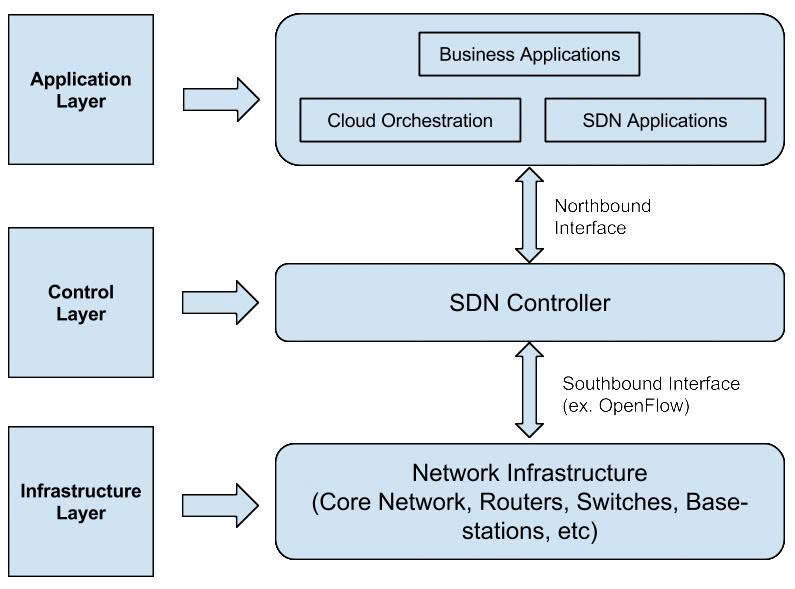
\includegraphics[width=0.60\textwidth]{image/SDN_ARCHITECTURE.jpg}
    \caption{Kiến trúc tổng quan của SDN}
    \label{fig:sdn_architecture}
\end{figure}

Lớp ứng dụng (Application Layer) là nơi triển khai các ứng dụng và dịch vụ mạng như giám sát, bảo mật, cân bằng tải, quản lý QoS, tối ưu băng thông hoặc tự động hóa cấu hình. Các ứng dụng này không trực tiếp cấu hình thiết bị mạng mà gửi yêu cầu đến SDN Controller thông qua giao diện northbound API. Nhờ đó, yêu cầu nghiệp vụ có thể được chuyển thành chính sách mạng cụ thể.

Lớp điều khiển (Control Layer) là thành phần trung tâm của SDN, thường được gọi là SDN Controller. Controller đóng vai trò như ``bộ não'' của mạng vì có khả năng thu thập thông tin topology, trạng thái liên kết, bảng luồng và chính sách vận hành. Dựa trên thông tin toàn cục này, Controller ra quyết định về định tuyến, phân bổ tài nguyên, kiểm soát truy cập hoặc chất lượng dịch vụ. Sau đó, Controller gửi chỉ thị xuống các thiết bị mạng thông qua giao diện southbound.

Lớp hạ tầng hoặc mặt phẳng dữ liệu (Infrastructure Layer/Data Plane) bao gồm các switch, router, firewall hoặc thiết bị mạng ảo. Nhiệm vụ chính của lớp này là chuyển tiếp gói tin theo các quy tắc đã được cài đặt trong bảng luồng. Các thiết bị ở lớp hạ tầng không cần tự xử lý toàn bộ logic điều khiển phức tạp mà tập trung vào việc thực thi nhanh và chính xác các quyết định do Controller đưa xuống.

\subsubsection{Nguyên lý hoạt động của SDN}

SDN hoạt động dựa trên cơ chế tách biệt giữa control plane và data plane. Khi một gói tin đi vào switch, thiết bị sẽ kiểm tra bảng luồng (flow table) để xác định cách xử lý. Nếu đã có quy tắc phù hợp, gói tin được chuyển tiếp, loại bỏ hoặc xử lý theo hành động đã định nghĩa. Nếu chưa có quy tắc, switch có thể gửi thông tin về gói tin hoặc luồng mới lên SDN Controller để xin quyết định xử lý.

\begin{figure}[H]
    \centering
    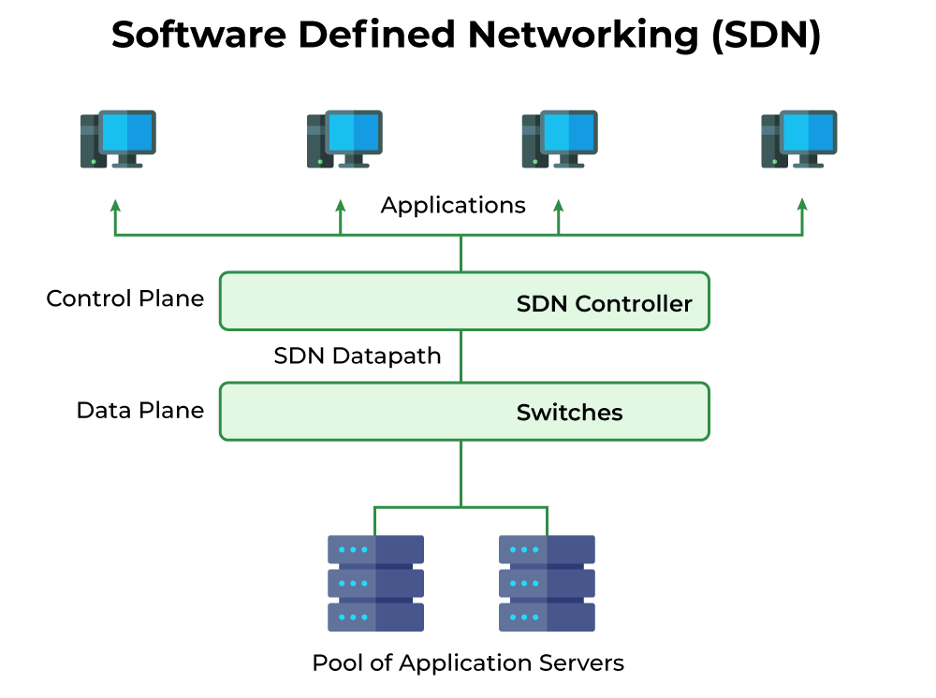
\includegraphics[width=0.80\textwidth]{image/nguyenlyhoatdongsdn.png}
    \caption{Nguyên lý hoạt động của SDN}
    \label{fig:nguyen_ly_hoat_dong_sdn}
\end{figure}

Sau khi nhận yêu cầu, Controller phân tích thông tin gói tin, trạng thái mạng và chính sách đang áp dụng. Controller có thể quyết định đường đi tối ưu, áp dụng chính sách bảo mật, giới hạn băng thông hoặc ưu tiên một loại lưu lượng nhất định. Quyết định này được chuyển lại cho switch dưới dạng quy tắc mới. Từ thời điểm đó, các gói tin cùng loại có thể được xử lý trực tiếp tại switch mà không cần hỏi Controller lặp lại, giúp giảm độ trễ và tăng hiệu quả chuyển tiếp.

Trong môi trường Campus, nguyên lý này cho phép hệ thống thay đổi chính sách theo trạng thái mạng hoặc theo nhóm người dùng. Ví dụ, Controller có thể ưu tiên lưu lượng học trực tuyến, giới hạn lưu lượng từ VLAN khách, cô lập một thiết bị có dấu hiệu bất thường hoặc điều chỉnh đường đi khi một liên kết bị nghẽn. Điều này giúp mạng phản ứng linh hoạt hơn so với mô hình cấu hình tĩnh truyền thống.

\subsubsection{Các giao thức và giao diện trong SDN}

OpenFlow là giao thức southbound phổ biến trong các mô hình SDN, cho phép Controller cài đặt, sửa đổi hoặc xóa các quy tắc trong bảng luồng của switch. Thông qua OpenFlow, Controller có thể quy định cách thiết bị xử lý gói tin dựa trên địa chỉ MAC, địa chỉ IP, cổng TCP/UDP, VLAN ID hoặc các trường tiêu đề khác. Đây là nền tảng quan trọng để SDN điều khiển lưu lượng ở mức chi tiết.

Bên cạnh OpenFlow, SDN còn có thể sử dụng nhiều cơ chế giao tiếp khác tùy theo thiết bị và nền tảng triển khai. Một số hệ thống dùng REST API, NETCONF, gRPC, SNMP hoặc giao diện dòng lệnh được tự động hóa để quản lý thiết bị mạng. Ở chiều ngược lại, northbound API giúp các ứng dụng quản trị, giám sát, bảo mật hoặc tự động hóa gửi yêu cầu chính sách đến Controller. Nhờ các giao diện này, SDN có thể tích hợp với hệ thống quản lý mạng, nền tảng giám sát, công cụ DevOps hoặc các dịch vụ đám mây.

Đối với đề tài, các giao thức và giao diện trong SDN có ý nghĩa quan trọng vì chúng là cầu nối giữa chính sách quản trị tập trung và thiết bị mạng Campus. Controller có thể thu thập trạng thái mạng, nhận biết liên kết, quản lý luồng dữ liệu và triển khai chính sách cho từng VLAN hoặc từng nhóm dịch vụ mà không cần cấu hình thủ công trên toàn bộ thiết bị.

\subsubsection{Phân loại mô hình SDN}

SDN có thể được triển khai theo nhiều mô hình khác nhau. Open SDN là mô hình sử dụng giao thức mở như OpenFlow để Controller điều khiển trực tiếp hành vi chuyển tiếp của switch. Mô hình này phù hợp với môi trường nghiên cứu, thử nghiệm hoặc các hệ thống cần kiểm soát chi tiết luồng dữ liệu.

SDN thông qua API là mô hình tận dụng các giao diện lập trình do thiết bị mạng cung cấp. Thay vì thay đổi hoàn toàn cơ chế chuyển tiếp của thiết bị, Controller hoặc hệ thống quản lý sử dụng API như REST API, NETCONF hoặc các công cụ tự động hóa để cấu hình thiết bị từ xa. Mô hình này phù hợp với môi trường có nhiều thiết bị sẵn có và cần chuyển đổi từng bước sang quản lý tập trung.

SDN dựa trên hypervisor tập trung vào ảo hóa mạng trong trung tâm dữ liệu hoặc môi trường cloud. Các mạng ảo, switch ảo và chính sách kết nối giữa máy ảo được tạo và quản lý trên lớp ảo hóa mà không cần thay đổi quá nhiều hạ tầng vật lý. Ngoài ra, mô hình Hybrid SDN kết hợp mạng truyền thống với SDN, trong đó một phần thiết bị vẫn vận hành theo cơ chế cũ, còn một phần được điều khiển bởi Controller. Đây là hướng phù hợp cho tổ chức muốn tận dụng hạ tầng hiện có và giảm chi phí chuyển đổi ban đầu.

\subsubsection{Ưu và nhược điểm của SDN}

Ưu điểm lớn nhất của SDN là khả năng quản lý tập trung. Controller cung cấp một điểm điều khiển chung cho toàn mạng, giúp giảm sai sót khi cấu hình thủ công và hỗ trợ triển khai chính sách nhất quán. SDN cũng tăng tính linh hoạt vì quản trị viên có thể thay đổi đường đi, cập nhật ACL, điều chỉnh QoS hoặc bổ sung dịch vụ mới thông qua phần mềm.

SDN còn hỗ trợ tối ưu hóa tài nguyên và hiệu năng mạng. Nhờ có cái nhìn tổng thể về topology và trạng thái liên kết, Controller có thể lựa chọn đường đi phù hợp, phân bổ băng thông hiệu quả hơn và giảm tình trạng nghẽn mạng. Khả năng tự động hóa cũng giúp rút ngắn thời gian triển khai dịch vụ, hỗ trợ mở rộng hệ thống và tích hợp với các công nghệ hiện đại như điện toán đám mây, NFV, IoT hoặc SD-WAN.

Tuy nhiên, SDN cũng tồn tại một số hạn chế. Controller là thành phần trung tâm nên nếu không được bảo vệ và dự phòng tốt, nó có thể trở thành điểm lỗi hoặc mục tiêu tấn công quan trọng. Việc triển khai SDN cũng đòi hỏi nhân sự có kiến thức về mạng, lập trình, API và bảo mật. Ngoài ra, sự khác biệt giữa các nhà cung cấp thiết bị có thể gây khó khăn khi tích hợp trong môi trường đa hãng. Chi phí đầu tư ban đầu cho Controller, thiết bị tương thích và đào tạo cũng là yếu tố cần cân nhắc.

\subsubsection{Ứng dụng thực tế của SDN}

SDN được ứng dụng rộng rãi trong trung tâm dữ liệu để quản lý lưu lượng quy mô lớn, tự động hóa cấu hình mạng ảo và triển khai chính sách bảo mật nhanh chóng. Trong mạng đám mây, SDN hỗ trợ tạo mạng ảo cho nhiều người thuê, cô lập tài nguyên và mở rộng dịch vụ linh hoạt. Trong mạng doanh nghiệp, SDN giúp đơn giản hóa quản trị. 

Đối với mạng Campus, SDN có thể được sử dụng để quản lý tập trung các VLAN, áp dụng chính sách truy cập theo nhóm người dùng, giám sát trạng thái liên kết, ưu tiên lưu lượng quan trọng và hỗ trợ phát hiện bất thường. Trong phạm vi đề tài, SDN không thay thế hoàn toàn mô hình Core--Distribution--Access mà đóng vai trò là lớp điều phối và quản lý tập trung. Hạ tầng phân cấp vẫn đảm nhiệm tổ chức vật lý và logic của mạng, trong khi SDN Controller giúp triển khai chính sách nhất quán, giảm cấu hình thủ công và hỗ trợ vận hành mạng Campus hiệu quả hơn.

\subsection{Công nghệ SD-WAN}

\begin{figure}[H]
    \centering
    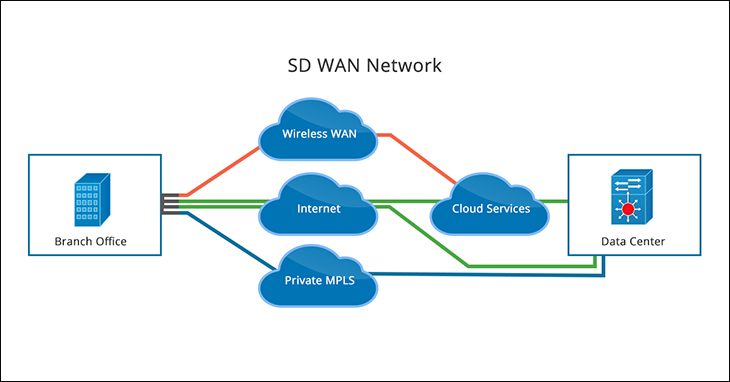
\includegraphics[width=0.80\textwidth]{image/sdwan.jpg}
    \caption{Minh họa công nghệ SD-WAN}
    \label{fig:sdwan}
\end{figure}

SD-WAN là công nghệ mạng diện rộng được điều khiển bằng phần mềm, cho phép quản lý tập trung các kết nối WAN giữa nhiều địa điểm. Thay vì phụ thuộc hoàn toàn vào một đường truyền riêng, SD-WAN có thể kết hợp nhiều loại kết nối như Internet, leased line hoặc 4G/5G và lựa chọn đường truyền phù hợp dựa trên chính sách, chất lượng đường truyền.

Trong môi trường trường đại học có nhiều cơ sở, SD-WAN giúp kết nối Campus chính với các cơ sở phụ, trung tâm dữ liệu hoặc dịch vụ đám mây một cách linh hoạt hơn. Hệ thống có thể ưu tiên lưu lượng quan trọng như hệ thống quản lý đào tạo, họp trực tuyến hoặc truy cập máy chủ nội bộ qua đường truyền có độ trễ thấp; trong khi lưu lượng thông thường có thể đi qua đường Internet chi phí thấp hơn. Khi một đường truyền gặp sự cố, SD-WAN có thể chuyển lưu lượng sang đường thay thế để duy trì kết nối.

Một thành phần quan trọng của SD-WAN là chính sách điều hướng lưu lượng theo ứng dụng. Chính sách này có thể dựa trên độ trễ, jitter, tỷ lệ mất gói, băng thông còn lại hoặc yêu cầu SLA. Nhờ đó, hệ thống không chỉ dự phòng ở mức kết nối mà còn tối ưu trải nghiệm người dùng. Bên cạnh đó, SD-WAN thường hỗ trợ mã hóa đường truyền, quản lý tập trung và hiển thị trạng thái kết nối giữa các site.

Trong phạm vi đề tài, SD-WAN được định hướng sử dụng cho bài toán kết nối nhiều cơ sở đào tạo. Mạng Campus tại cơ sở chính cung cấp các dịch vụ dùng chung, còn cơ sở phụ cần truy cập ổn định và an toàn đến các dịch vụ này. Khi kết hợp với SDN, SD-WAN giúp mở rộng quản trị từ mạng nội bộ ra WAN.
